%----------------Cap_03----------------%
\chapter{Metodologia e Desenvolvimento do Sistema}
\label{cap:metodologia}
 
Este capítulo apresenta o detalhamento completo da fase experimental do projeto, cobrindo a descrição do sistema físico, a modelagem e identificação do modelo dinâmico e a implementação do controlador no hardware embarcado. A arquitetura da solução está sintetizada no diagrama de blocos da Figura~\ref{fig:diagrama-blocos-projeto}, que organiza o desenvolvimento em duas fases.
 
\begin{figure}[H]
    \centering
    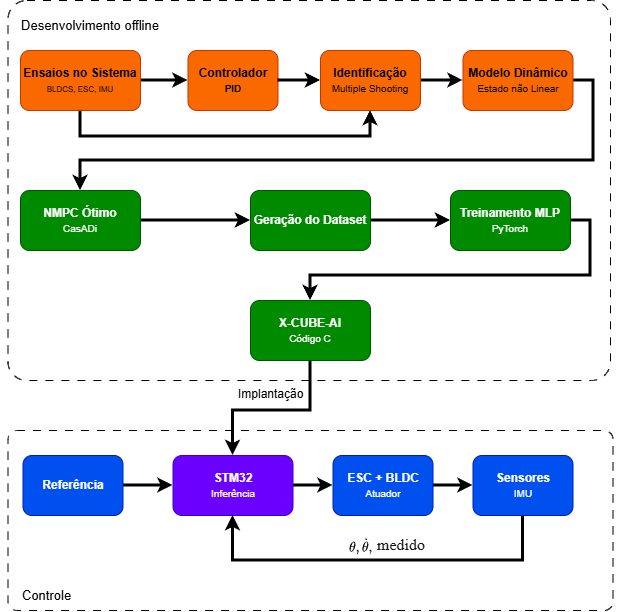
\includegraphics[width=1\textwidth]{img/blocos-projeto.png}
    \caption{Diagrama de Blocos do Projeto}
    \label{fig:diagrama-blocos-projeto}
\end{figure}

 A fase offline corresponde: (i)~a síntese e implantação do controlador PID em malha fechada, utilizado tanto para estabilizar a planta durante a coleta de dados quanto como referência de desempenho na comparação final (Seção~\ref{sec:pid}); (ii)~a aquisição dos dados de identificação em malha fechada com o PID ativo e a estimação dos parâmetros do modelo dinâmico via \textit{multiple shooting} (Seção~\ref{sec:identificacao}); (iii)~a formulação e resolução do NMPC via CasADi, a geração do \textit{dataset} e o treinamento da rede neural MLP (Seção~\ref{sec:sintese}). A fase de operação em tempo real, na parte inferior, corresponde à implantação do controlador embarcado no STM32 e sua atuação sobre a planta física (Seção~\ref{sec:embarcado}). A Seção~\ref{sec:descricao_fisica} descreve a bancada e os componentes de hardware que suportam ambas as fases.
 
% ------------------------------------------------------------
\section{Descrição do Sistema Físico}
\label{sec:descricao_fisica}
A infraestrutura física e mecânica da bancada do aeropêndulo utilizada neste trabalho foi originalmente projetada e construída por \citeonline{lima2025}. O sistema mecânico pré-existente e reaproveitado compreende a base de madeira, as torres de suporte, o eixo de alumínio instrumentado e a haste pendular contendo o motor \textit{brushless} (BLDC) acoplado.

O aeropêndulo atua como um sistema de um grau de liberdade, composto por esse braço rígido livre para rotacionar em torno do eixo horizontal fixo. A posição angular $\theta$ é medida em relação à horizontal, sendo $0^\circ$ definido quando o sistema está em repouso com o motor na posição inferior.

% ------------------------------------------------------------
\subsection{Estrutura Mecânica}

A estrutura física do aeropêndulo é montada sobre uma base de madeira compensada. Dois suportes triangulares confeccionados em MDF sustentam o eixo de rotação do sistema. As faces foram unidas por colagem nas arestas, e peças impressas em 3D foram fixadas nos cantos de cada torre e parafusadas à base.

Para fixar o eixo de alumínio às torres, é utilizado um cuboide retangular contendo um rolamento de esferas, permitindo que o eixo gire livremente. No centro do eixo foi usinado e rosqueado um furo para encaixe da haste do pêndulo.

A haste rosqueada também permite a fixação e remoção facilitada de contrapesos, que foram usinados e rosqueados para se encaixar diretamente na haste. Um suporte impresso em 3D acopla o motor BLDC à extremidade da haste. A propulsão é gerada por uma hélice bipá de passo fixo. Um alojamento impresso em 3D para a Unidade de Medição Inercial (IMU) foi desenvolvido e fixado ao eixo de rotação, responsável por capturar o ângulo do sistema. A Figura~\ref{fig:montagem-bancada} ilustra o formato atual da bancada. Os principais parâmetros construtivos do sistema são resumidos na Tabela~\ref{tab:componentes_mecanicos}.

\begin{figure}[h]
    \centering
    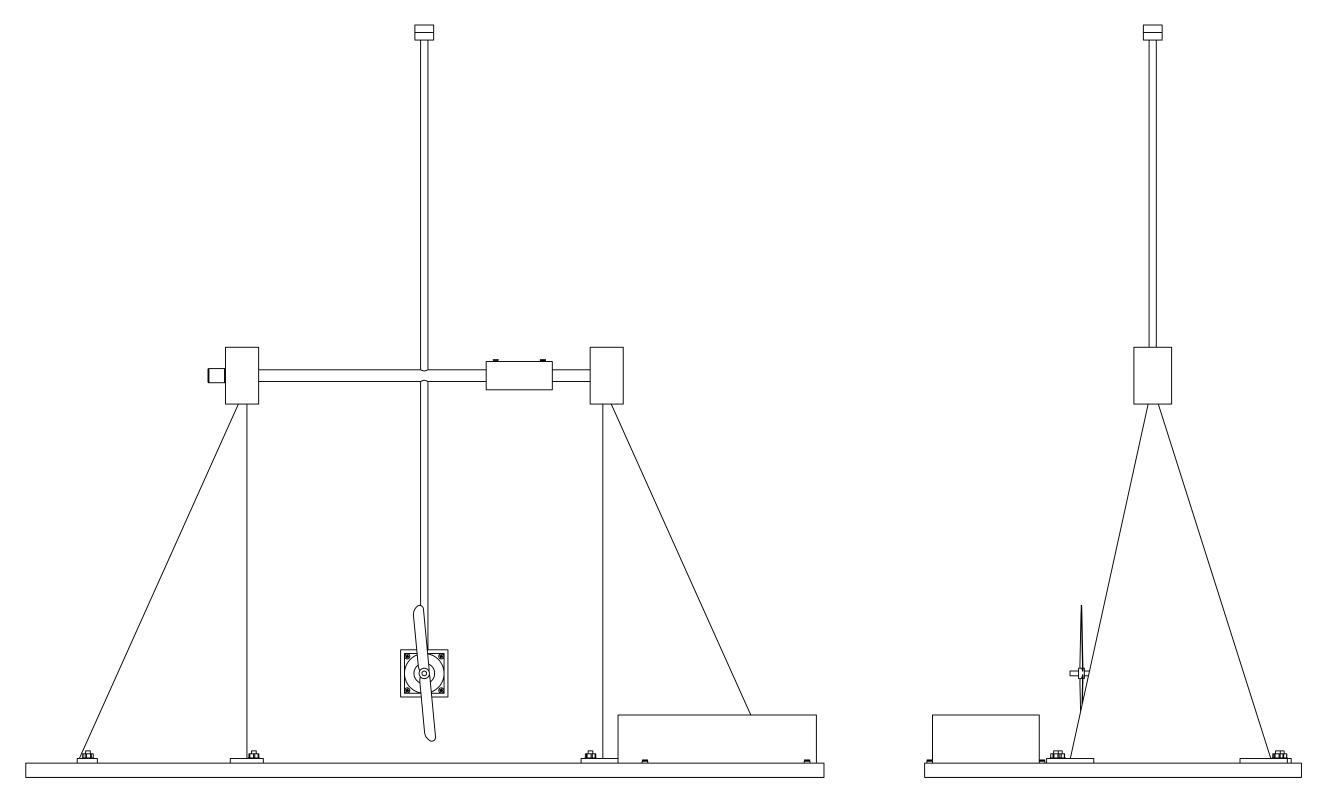
\includegraphics[width=1\textwidth]{img/montagem-bancada.png}
    \caption{Desenho da Bancada}
    \label{fig:montagem-bancada}
\end{figure}

\begin{table}[h!]
    \centering
    \caption{Componentes mecânicos do aeropêndulo}
    \label{tab:componentes_mecanicos}
    \begin{tabular}{ll}
        \hline
        \textbf{Componente}       & \textbf{Material / Modelo}              \\
        \hline
        Base                      & Madeira compensada                      \\
        Torres de suporte         & MDF com reforços em PLA (impressão 3D)  \\
        Eixo de rotação           & Alumínio                                \\
        Mancal                    & Rolamento de esferas                    \\
        Haste do pêndulo          & Haste rosqueada                         \\
        Contrapesos               & Peças rosqueadas (ajustáveis)           \\
        Suporte do motor          & PLA (impressão 3D)                      \\
        Alojamento da IMU         & PLA (impressão 3D)                      \\
        Motor                     & EMAX RS2306                             \\
        Hélice                    & Bipá, passo fixo                        \\
        \hline
    \end{tabular}
\end{table}

% ------------------------------------------------------------
\subsection{Sensores}

% ------------------------------------------------------------
\subsubsection{Unidade de Medição Inercial (IMU)}

A unidade de medição inercial utilizada é o ICM-20948, fabricado pela InvenSense (TDK), um dispositivo MEMS de 9 eixos que integra giroscópio triaxial, acelerômetro triaxial e magnetômetro triaxial em um único encapsulamento QFN de 3$\times$3$\times$1\,mm \cite{invensense2021icm20948}.

A comunicação com o microcontrolador é realizada via I$^2$C no modo \textit{fast} (400\,kHz), utilizando os pinos SCL e SDA do STM32. O endereço I$^2$C do dispositivo é definido pelo nível lógico do pino AD0, com AD0 em nível baixo, o endereço é \texttt{0x68}. Os dados do giroscópio e do acelerômetro são utilizados em conjunto na estimação do ângulo gerado pelo braço do aeropêndulo.

O giroscópio apresenta fundo de escala programável de $\pm250$, $\pm500$, $\pm1000$ ou $\pm2000$\,dps, com ADC de 16 bits e sensibilidade de 131\,LSB/dps na configuração de menor fundo de escala. A densidade espectral de ruído típica é de 0,015\,dps/$\sqrt{\text{Hz}}$, e o filtro passa-baixas digital (DLPF) é configurável entre 5,7 e 197\,Hz \cite{invensense2021icm20948}. A Tabela~\ref{tab:icm_gyro} resume os parâmetros do giroscópio que são relevantes para a aplicação.

\begin{table}[h]
    \centering
    \caption{Parâmetros do giroscópio do ICM-20948 utilizados no projeto.}
    \label{tab:icm_gyro}
    \begin{tabular}{lcc}
        \hline
        \textbf{Parâmetro} & \textbf{Valor} & \textbf{Unidade} \\
        \hline
        Fundo de escala selecionado & $\pm500$ & dps \\
        Sensibilidade                & 65,5   & LSB/dps \\
        Resolução do ADC             & 16     & bits \\
        Frequência de amostragem     & 100    & Hz \\
        Largura de banda do DLPF     & 51,2   & Hz \\
        Interface de comunicação     & I$^2$C & {-} \\
        Tensão de alimentação (VDD)  & 3,3    & V \\
        \hline
    \end{tabular}
\end{table}

A frequência de amostragem de 100\,Hz satisfaz o requisito de $T_s \leq 10$\,ms imposto pela dinâmica do aeropêndulo, e a largura de banda do filtro de 51,2\,Hz é suficiente para capturar os modos dinâmicos relevantes sem amplificar ruído de alta frequência.

A leitura dos registradores de saída do giroscópio é executada via interrupção de timer no STM32, garantindo periodicidade determinística.

% ------------------------------------------------------------
\subsection{Microcontrolador STM32 Nucleo-F446RE}

O núcleo de processamento do aeropêndulo é composto pelo microcontrolador STM32F446, baseado na arquitetura Arm Cortex-M4 de 32 bits, operando a uma frequência de clock máxima de 180\,MHz. Este processador incorpora uma Unidade de Ponto Flutuante (FPU) em hardware que suporta todas as instruções de precisão única do padrão IEEE 754, o que elimina a sobrecarga computacional de emulação por software e otimiza a execução em tempo real do algoritmo de controle do aeropêndulo e da filtragem dos sensores. A arquitetura de memória do dispositivo conta com 512\,KB de memória Flash para armazenamento do firmware e 128\,KB de memória SRAM para alocação dinâmica de variáveis e buffers de execução \cite{stm32}.

Os periféricos internos atendem aos requisitos dinâmicos e de interface do sistema, dividindo-se nas seguintes funções:

\begin{itemize}
    \item \textbf{Inter-Integrated Circuit (I$^2$C):} Barramento serial síncrono configurado no modo \textit{Fast Mode} (400\,kHz) para comunicação direta com a IMU ICM-20948, realizando a leitura periódica dos registradores do acelerômetro e giroscópio.
    \item \textbf{Temporizador (TIM):} Configurado em modo de geração de PWM (\textit{Pulse Width Modulation}) com resolução adequada para o acionamento do ESC (\textit{Electronic Speed Controller}), regulando de forma determinística a potência elétrica entregue ao motor \textit{brushless}.
    \item \textbf{Universal Asynchronous Receiver-Transmitter (UART):} Interface serial assíncrona estabelecida com taxa de transmissão elevada (ex.: 500.000\,baud) para o envio de telemetria em tempo real (ângulo estimado, erro, ação de controle) para o computador de ensaios e recepção de comandos de depuração.
\end{itemize}

A Tabela~\ref{tab:perifericos_stm32} especifica a atribuição física de pinos e periféricos utilizada na implementação do protótipo.

\begin{table}[h]
    \centering
    \caption{Mapeamento de periféricos e pinos do STM32F446 para o aeropêndulo.}
    \label{tab:perifericos_stm32}
    \begin{tabularx}{\textwidth}{llXX}
        \hline
        \textbf{Periférico} & \textbf{Pino} & \textbf{Função Configurada} & \textbf{Destino / Interface} \\
        \hline
        \\
        I2C1\_SCL  & PB8  & Clock do barramento I$^2$C (400\,kHz) & Pino SCL da IMU ICM-20948 \\
        I2C1\_SDA  & PB9  & Dados do barramento I$^2$C (400\,kHz) & Pino SDA da IMU ICM-20948 \\
        TIM1\_CH1  & PA8  & Saída PWM (Sinal de Controle) & Entrada de Sinal do ESC \\
        USART2\_TX & PA2  & Transmissão Serial Assíncrona & Receptor USB-UART \\
        USART2\_RX & PA3  & Recepção Serial Assíncrona    & Receptor USB-UART \\
        \hline
    \end{tabularx}
\end{table}

A Figura~\ref{fig:esquematico} apresenta o esquemático elétrico simplificado da bancada, ilustrando a interligação entre o STM32 Nucleo-F446RE, a IMU ICM-20948 e o ESC. A fonte de alimentação do motor (VBAT) é independente da 
alimentação lógica do microcontrolador.

\begin{figure}[h]
    \centering
    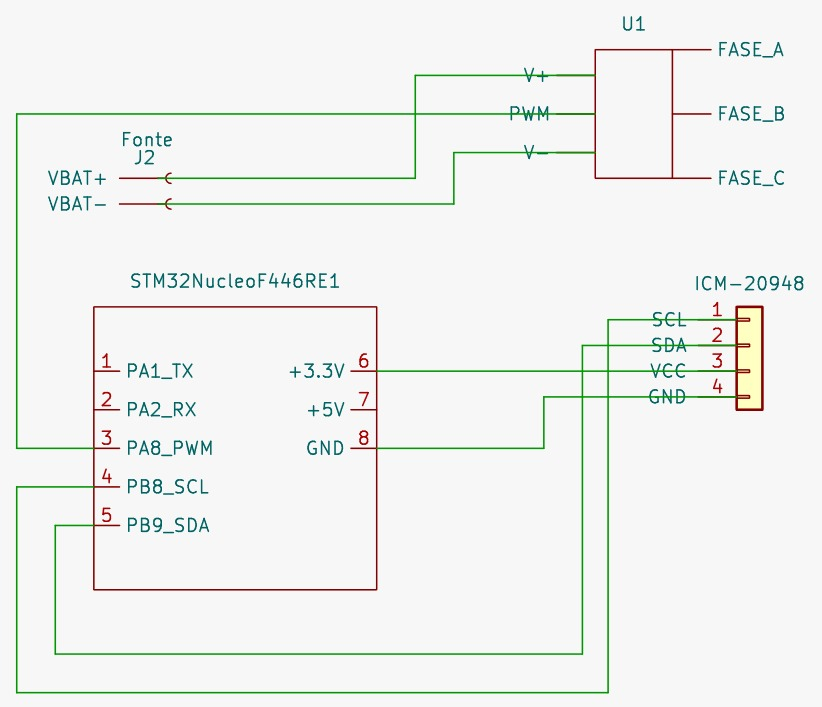
\includegraphics[width=1\textwidth]{img/diagrama-eletrico.png}
    \caption{Esquemático elétrico simplificado da bancada}
    \label{fig:esquematico}
\end{figure}

% ============================================================
\section{Identificação do Modelo Dinâmico}
\label{sec:identificacao}

A síntese do Controle Preditivo Não-Linear (NMPC) exige um modelo matemático rigoroso, mas a modelagem puramente analítica do aeropêndulo impõe dificuldades práticas, visto que parâmetros físicos são de difícil mensuração isolada e o arranjo motor-hélice introduz não-linearidades que costumam ser ignoradas. Contudo, as abordagens clássicas de identificação baseadas em modelos lineares possuem restrições estruturais que as tornam insuficientes para representar os efeitos aerodinâmicos em todo o envelope operacional da planta \cite{jiang2022}. 

Diante dessas limitações, adota-se uma abordagem híbrida: a estrutura do modelo é derivada analiticamente a partir dos princípios físicos do sistema, enquanto os parâmetros de difícil mensuração são estimados por identificação experimental. Pela Segunda Lei de Newton aplicada à dinâmica rotacional, considerando  explicitamente a massa do conjunto motor-hélice $m_1$ posicionada à distância  $L_1$ do pivô e a massa do contrapeso $m_2$ posicionada à distância $L_2$ no  lado oposto, a equação de movimento do aeropêndulo é:

\begin{equation}
    J\ddot{\theta} + b\dot{\theta} + (m_1 L_1 - m_2 L_2)\,g\sin(\theta) = \tau(u),
    \label{eq:dinamica}
\end{equation}
\noindent onde $\theta$ é o ângulo de inclinação em relação à vertical,  $\dot{\theta}$ a velocidade angular, $J$ o momento de inércia total, $b$ o  coeficiente de atrito viscoso, $g$ a aceleração da gravidade e $\tau(u)$ o  torque gerado pelo empuxo do motor em função do sinal de controle $u$. O termo  $(m_1 L_1 - m_2 L_2)\,g\sin(\theta)$ caracteriza a não-linearidade gravitacional  intrínseca ao sistema, cujo valor efetivo depende do balanço entre o torque  restaurador do motor e o torque compensatório do contrapeso, tornando inadequada  qualquer representação linear para operação em ampla faixa angular \cite{khalil2002}.

Para o formalismo do NMPC, é necessário representar o sistema na forma de  espaço de estados não-linear $\dot{x} = f(x, u)$. Definindo o vetor de estados  $x = [\theta,\;\dot{\theta}]^\top$ e isolando $\ddot{\theta}$ na  Equação~\ref{eq:dinamica}, obtém-se:

\begin{equation}
    \dot{x} = f(x,\, u) =
    \begin{bmatrix}
        \dot{\theta} \\[4pt]
        \dfrac{\tau(u) - b\dot{\theta} - (m_1 L_1 - m_2 L_2)\,g\sin(\theta)}{J}
    \end{bmatrix},
    \label{eq:estadonl}
\end{equation}
\noindent forma exigida pelo NMPC para propagar os estados ao longo do horizonte de predição \cite{mayne2000}. Os parâmetros geométricos e de massa ($m_1$, $m_2$,  $L_1$ e $L_2$) são medidos fisicamente e fixados no modelo. Os parâmetros $J$,  $b$ e a constante de empuxo $K_\tau$, assumindo $\tau(u) = K_\tau u$, não são  diretamente mensuráveis de forma isolada e são estimados por identificação  experimental, conforme descrito nas subseções seguintes.

% ------------------------------------------------------------
\subsection{Ensaios e Estratégia de Excitação}
\label{subsec:ensaios}

Os ensaios de identificação foram conduzidos com o aeropêndulo operando obrigatoriamente em malha fechada, estabilizado por um controlador PID preliminar embarcado no microcontrolador STM32 (Seção~\ref{sec:pid}). A realimentação em malha fechada constituiu um requisito mandatório de segurança operacional: dada a natureza subamortecida da planta e a ausência de batentes amortecidos, ensaios em malha aberta conduziriam o braço do pêndulo a colisões destrutivas contra os limites físicos da bancada ou a regimes de saturação irreversível do atuador.

O microcontrolador STM32 Nucleo-F446RE foi responsável pela execução determinística da lei de controle PID a uma taxa de amostragem de $f_s = 100$\,Hz ($T_s = 10$\,ms), pela injeção sincronizada dos sinais de referência dinâmicos e pelo envio contínuo da telemetria serial em tempo real para a estação de processamento em terra.

\subsubsection{Sinais de Excitação}

A identificação precisa da planta exige sinais de excitação com elevada riqueza espectral (\textit{persistently exciting}), capazes de estimular simultaneamente os múltiplos fenômenos dinâmicos acoplados: o comportamento não-linear de empuxo do conjunto propulsor, o atraso de transporte eletromecânico, o amortecimento viscoso e a componente gravitacional dependente da inclinação angular descrita pelo termo $(m_1 L_1 - m_2 L_2)g\sin(\theta)$.

Para assegurar a identificabilidade desses efeitos em todo o envelope físico, estabeleceram-se as seguintes premissas metodológicas de projeto dos sinais:

\begin{enumerate}
    \item \textbf{Frequência máxima de excitação ($f_{\max} = 0{,}50$\,Hz):} A largura de banda mecânica do aeropêndulo é dominada por polos lentos associados à inércia da haste e aos tempos de subida do empuxo aerodinâmico. Fixou-se, portanto, a frequência máxima de excitação em $f_{\max} = 0{,}50$\,Hz. Frequências superiores a esse patamar não acrescentam informações dinâmicas relevantes sobre o movimento de corpo rígido do aeropêndulo.
    
    \item \textbf{Dois níveis de estabilização em malha fechada ($45^\circ$ e $60^\circ$):} Os ensaios foram realizados em torno de dois pontos de equilíbrio centrais: $\theta_0 = 45^\circ$ e $\theta_0 = 60^\circ$. A operação em dois patamares distintos é indispensável para cobrir diferentes inclinações operacionais da planta, onde o ganho estático requerido do motor e as derivadas do torque gravitacional diferem substancialmente. Em $45^\circ$, o sistema opera na região de máxima sensibilidade gravitacional ($\frac{d}{d\theta}\sin\theta = \cos 45^\circ \approx 0{,}707$), enquanto em $60^\circ$ o empuxo contínuo exigido para sustentação estática é cerca de $22\%$ superior, alterando o ponto de trabalho do propulsor.
    
    \item \textbf{Faixa total definida de referência ($0^\circ$ a $120^\circ$):} O envelope total de rastreamento estipulado para o projeto compreende o intervalo de $0^\circ$ (posição de repouso vertical com o motor inferior desativado) até $120^\circ$ (inclinação acentuada acima da horizontal). Em torno do nível de $45^\circ$, os sinais dinâmicos impõem variações de até $\pm 45^\circ$, cobrindo o intervalo de $0^\circ$ a $90^\circ$. Em torno do nível de $60^\circ$, os sinais atingem excursões de até $\pm 60^\circ$, percorrendo de $0^\circ$ a $120^\circ$, de modo a excitar toda a não-linearidade do envelope de voo.
\end{enumerate}


A Tabela~\ref{tab:ranges_angulos} sintetiza a matriz experimental dos 24 sinais sintetizados para a bancada, estruturados em torno dos patamares de $45^\circ$ e $60^\circ$ para cobrir todo o envelope dinâmico ($0^\circ$ a $120^\circ$).

\begin{table}[H]
    \centering
    \caption{Matriz experimental dos sinais de excitação em malha fechada.}
    \label{tab:ranges_angulos}
    \begin{tabular}{l c p{7.5cm} c}
        \toprule
        \textbf{Classe do Sinal} & \textbf{Patamares} & \textbf{Configuração e Parâmetros} & \textbf{Ensaios} \\ \midrule
        Degraus Fixos   & $45^\circ$ e $60^\circ$ & Patamares com duração fixa de 4,0\,s & 6 \\
        APRBS           & $45^\circ$ e $60^\circ$ & Chaveamento aleatório entre 2,0 e 4,0\,s & 6 \\
        Chirp (\textit{Swept-Sine}) & $45^\circ$ e $60^\circ$ & Varredura de 0,05 a 0,50\,Hz (amplitudes $\pm 25^\circ$ a $\pm 60^\circ$) & 6 \\
        Multisseno      & $45^\circ$ e $60^\circ$ & Espectro uniforme com $f_{\max} \in \{0{,}30;\; 0{,}40;\; 0{,}50\}$\,Hz & 6 \\ \midrule
        \textbf{Total}  & \multicolumn{2}{l}{\textit{Total de 3 ensaios por patamar para cada classe}} & \textbf{24} \\ \bottomrule
    \end{tabular}
    \sourceTab{o autor, 2026.}
\end{table}



Para cumprir tais requisitos, a síntese dos perfis de referência foi realizada em ambiente computacional a uma taxa de amostragem de $f_s = 100$\,Hz ($T_s = 10$\,ms). Todas as trajetórias geradas incorporam intervalos iniciais e finais de repouso (\textit{zero-padding} de 3 a 5\,s), indispensáveis para a estabilização da comunicação serial e para a calibração automática de \textit{bias} do giroscópio da IMU antes do início da movimentação dinâmica. Adicionalmente, os perfis foram delimitados a valores não-negativos ($\ge 0^\circ$) para respeitar a geometria da bancada física, sendo estruturados em torno dos patamares operacionais de $45^\circ$ e $60^\circ$.

Foram sintetizadas quatro classes principais de sinais dinâmicos:

\begin{itemize}
    \item \textbf{Multi-seno com fases aleatórias:} Formado pela sobreposição harmônica de $d$ senoides com amplitude homogênea distribuídas uniformemente no espectro até $f_{\max} = 0{,}50$\,Hz, com fases $\varphi_k$ sorteadas independentemente em $[0, 2\pi)$:
    \begin{equation}
        r(t) = \theta_0 + \sum_{k=1}^{d} A_k \cos\!\bigl(2\pi f_k t + \varphi_k\bigr), \qquad f_k = \frac{k}{d} f_{\max}.
    \end{equation}
    A aleatorização das fases calculada no MATLAB minimiza o fator de crista temporal ($CF \le 1{,}8$), permitindo injetar alta densidade de potência sem provocar saturação nos atuadores \cite{ljung1999}.
    
    \item \textbf{\textit{Swept sine} (Chirp):} Senoide com frequência continuamente modulada de forma linear de $f_1 = 0{,}05$\,Hz até $f_2 = f_{\max} = 0{,}50$\,Hz. O ensaio varre de forma contínua o espectro em amplitudes controladas ($\pm 25^\circ$, $\pm 35^\circ$, $\pm 40^\circ$, $\pm 45^\circ$ e $\pm 60^\circ$), permitindo avaliar o comportamento dinâmico e o atraso de fase em função da frequência e amplitude.
    
    \item \textbf{Sequências de degraus (APRBS e múltiplos patamares):} Sinais de amplitude comutada pseudo-aleatória, conhecidos pela sigla APRBS (\textit{Amplitude Pseudo-Random Binary Sequence}), gerados com duração de chaveamento aleatória entre 2\,s e 4\,s, além de séries de degraus com patamares fixos. Esses sinais provocam saltos abruptos seguidos de trechos estacionários, estimulando os modos transitórios de aceleração e possibilitando a verificação direta do ganho em regime permanente.
    
    \item \textbf{Curva semi-estática:} Rampa suave de variação angular ascendente e descendente com longa duração ($T_f = 75$\,s), utilizada especificamente para levantar a característica estática de empuxo e quantificar os efeitos de histerese mecânica e atrito seco dos mancais.
\end{itemize}

\subsubsection{Particionamento dos Dados}
\label{subsec:divisao_dados}

Para garantir que o modelo identificado possua alta capacidade de generalização e não sofra de sobreajuste (\textit{overfitting}) a um padrão temporal particular, adotou-se um critério sistemático de particionamento dos dados experimentais coletados na bancada:

\begin{itemize}
    \item \textbf{Conjunto de Treinamento dos Modelos:} Foram selecionados exclusivamente os ensaios que apresentavam a maior frequência ($f_{\max} = 0{,}50$\,Hz) e as maiores amplitudes angulares em ambos os níveis de equilíbrio. Especificamente, o conjunto de treinamento é composto por 6 ensaios fundamentais:
    \begin{enumerate}
        \item Multisseno em $45^\circ$ com frequência máxima de $0{,}50$\,Hz;
        \item Chirp em $45^\circ$ com amplitude de $\pm 45^\circ$ (excursão de $0^\circ$ a $90^\circ$);
        \item Sequência APRBS em $45^\circ$;
        \item Multisseno em $60^\circ$ com frequência máxima de $0{,}50$\,Hz;
        \item Chirp em $60^\circ$ com amplitude de $\pm 60^\circ$ (excursão de $0^\circ$ a $120^\circ$);
        \item Sequência APRBS em $60^\circ$.
    \end{enumerate}
    Ao concentrar os ensaios de maior largura de banda e amplitude no treinamento, assegura-se que o algoritmo de estimação seja exposto às condições dinâmicas mais severas e às máximas deflexões não-lineares da bancada. A evolução temporal das referências angulares $r(t)$, dos ângulos medidos $\theta(t)$ e das respectivas ações de controle $u(t)$ aplicadas nos 6 ensaios de treinamento é apresentada na Figura~\ref{fig:sinais_treinamento}.
    
    \item \textbf{Conjunto de Validação Independente e Testes \textit{Free-Run}:} Todos os ensaios restantes coletados na bancada física foram estritamente reservados para validação cruzada independente. Este conjunto reúne sinais com menores frequências de excitação ($0{,}30$\,Hz e $0{,}40$\,Hz), menores amplitudes ($\pm 25^\circ$, $\pm 35^\circ$, $\pm 40^\circ$) e perfis distintos de degraus estacionários, tanto em $45^\circ$ quanto em $60^\circ$. A avaliação nesses dados testa a capacidade do modelo de interpolar dinâmicas, reproduzir fielmente a resposta em frequências intermediárias e manter predições estáveis em simulação livre (\textit{free-run}) recursiva de longo prazo sem divergência. A Figura~\ref{fig:sinais_validacao} ilustra os sinais correspondentes ao conjunto de ensaios de validação independente.
\end{itemize}

\begin{figure}[H]
    \centering
    \caption{Sinais de ensaios para treinamento.}
    \label{fig:sinais_treinamento}
    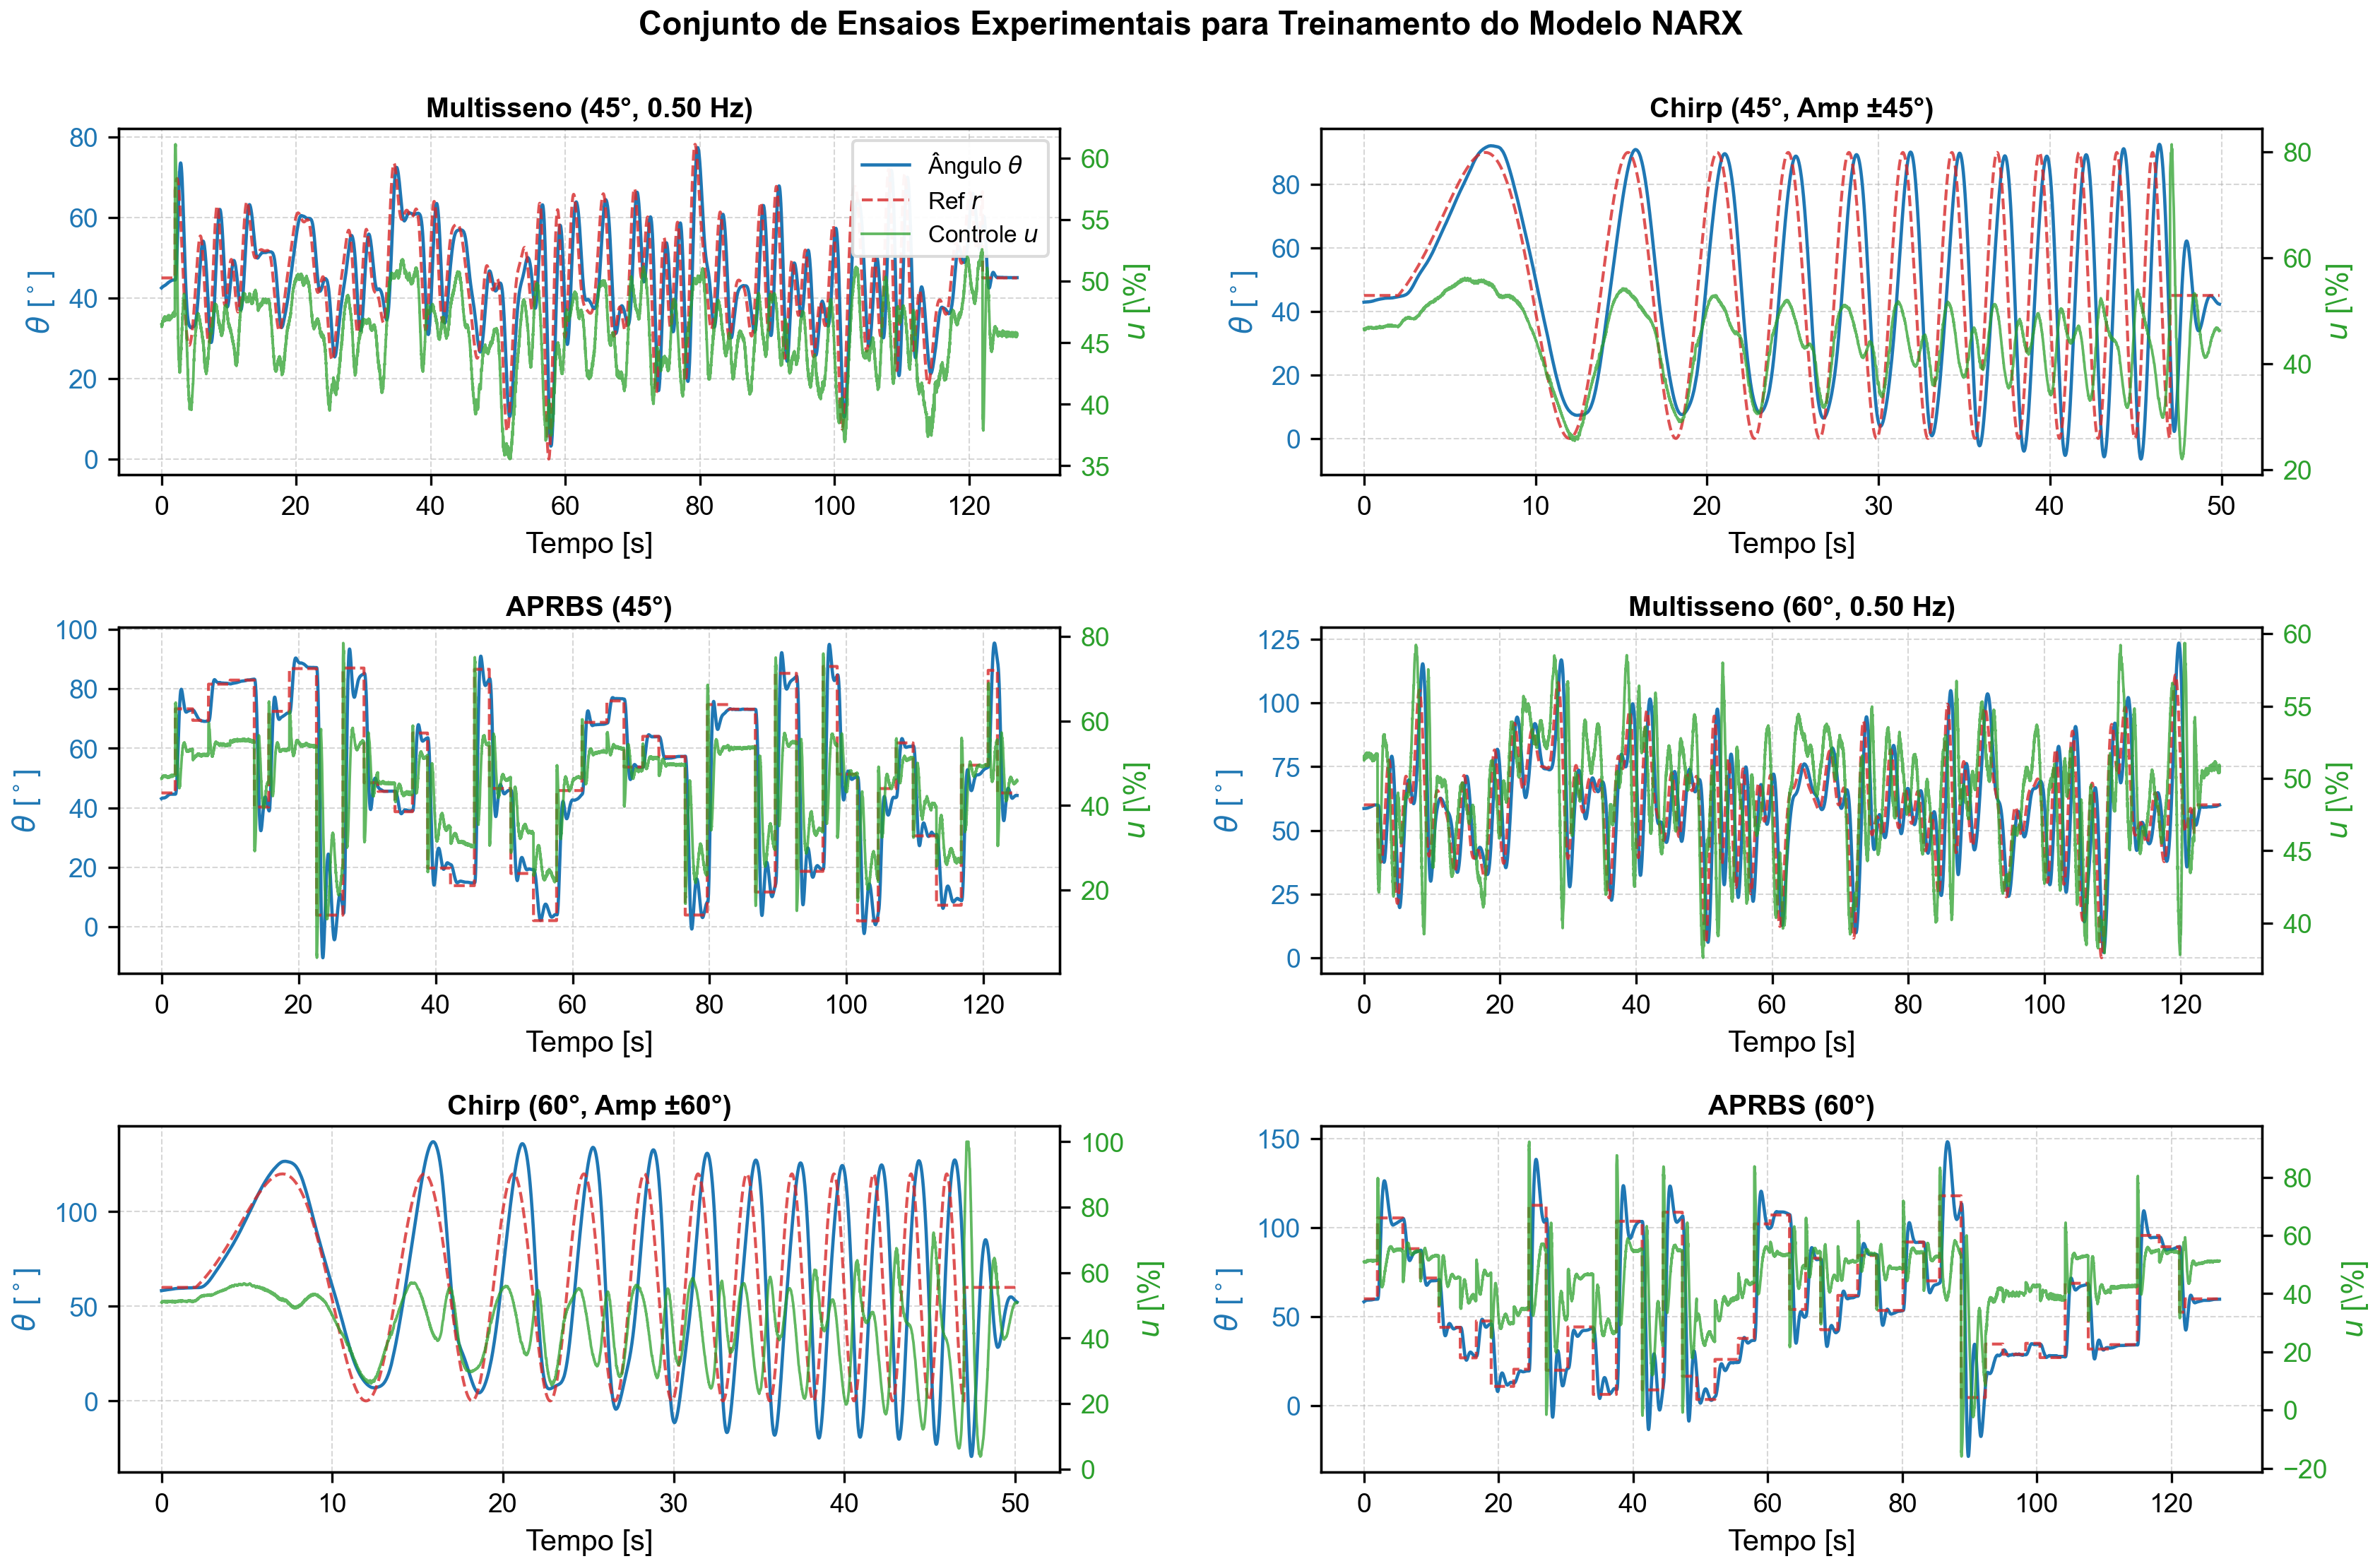
\includegraphics[width=0.90\textwidth]{img/resultados/narx_train_datasets.png}
    \sourceFig{o autor, 2026.}
\end{figure}

\begin{figure}[H]
    \centering
    \caption{Sinais de ensaios de validação independente.}
    \label{fig:sinais_validacao}
    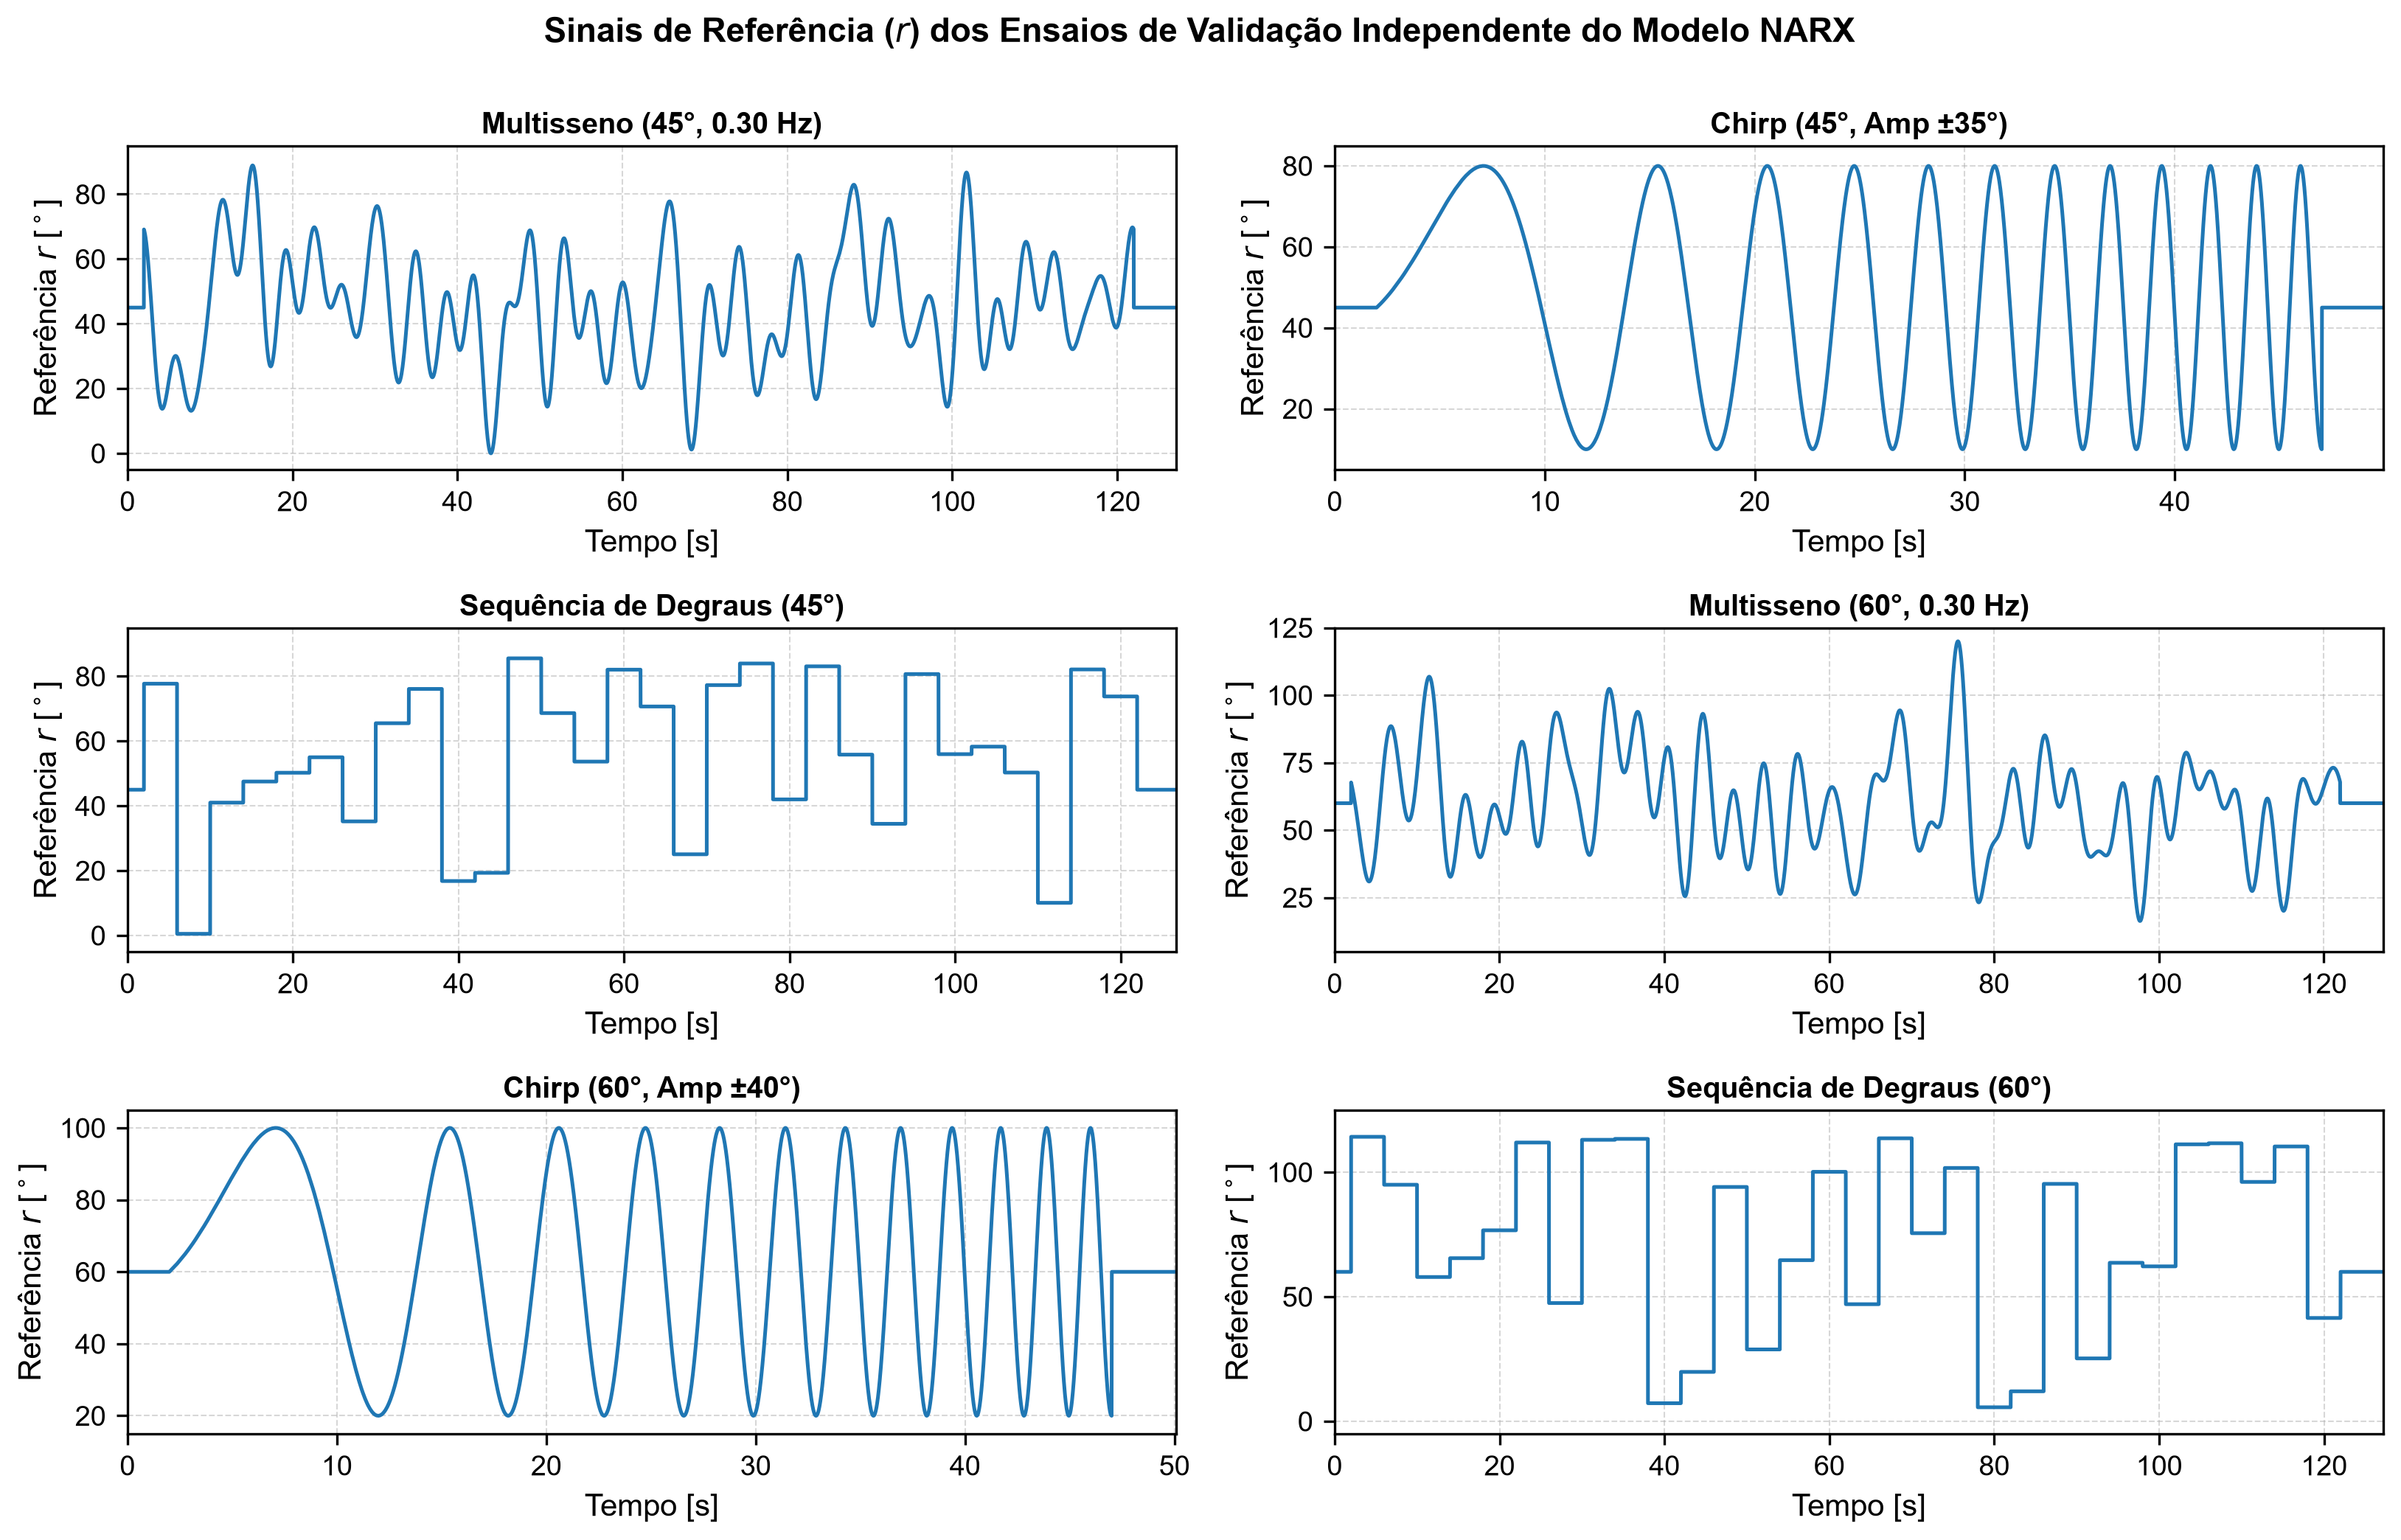
\includegraphics[width=0.90\textwidth]{img/resultados/narx_val_datasets.png}
    \sourceFig{o autor, 2026.}
\end{figure}

\subsubsection{Procedimento de Coleta de Dados}

Durante os ensaios, os dados foram transmitidos em tempo real pela interface USART2 do microcontrolador STM32 Nucleo-F446RE a uma taxa de comunicação de 500.000\,baud para o computador hospedeiro. Cada quadro de telemetria transmitido continha o carimbo de tempo determinístico (\textit{timestamp} com resolução de microssegundos), o sinal de referência $r(t)$, a ação de controle de saída $u(t)$ calculada pelo PID (expressa em porcentagem de \textit{duty cycle} do PWM no ESC) e o ângulo $\theta(t)$ estimado pelo filtro complementar a partir dos eixos do acelerômetro e giroscópio.

Os pacotes seriais foram capturados por um script Python dedicado utilizando a biblioteca \texttt{pyserial}, armazenados em arquivos estruturados de formato CSV e submetidos à rotina de pré-processamento, na qual os primeiros 10\,s (partida do motor e acomodação da comunicação) e os últimos 13\,s (desativação e frenagem) foram aparados, preservando os trechos estacionários de regime contínuo. O Algoritmo~\ref{alg:aquisicao_dados} sintetiza a lógica do laço em tempo real executada no microcontrolador durante as coletas.

\begin{algorithm}[H]
\caption{Ciclo Determinístico de Amostragem e Telemetria no STM32}
\begin{algorithmic}[1]
\label{alg:aquisicao_dados}
\Procedure{Setup}{}
    \State Inicializar periféricos (TIM, I$^2$C no modo Fast 400\,kHz, UART a 500\,kbaud, PWM a 50\,Hz)
    \State Calibrar offsets de bias do giroscópio da IMU ICM-20948 em repouso
    \State Inicializar estados internos do filtro complementar e integrador do PID
\EndProcedure

\Statex
\Procedure{Loop Amostragem Determinística}{}
    \State Aguardar comando de sincronização de ensaio via UART
    \State $t_{\text{inicio}} \gets \text{obterMicros()}$

    \While{$\text{ensaioAtivo}$}
        \State Sincronizar com período base do Timer de hardware ($T_s = 10\,\text{ms} \to 100\,\text{Hz}$)
        \State $t_{\text{atual}} \gets \text{obterMicros()} - t_{\text{inicio}}$

        \State Atualizar referência angular dinâmica: $\theta_{\text{ref}} \gets \text{avaliarSinalExcitacao}(t_{\text{atual}})$
        \State Ler acelerômetro ($a_x, a_z$) e giroscópio ($\omega_y$) da IMU via I$^2$C DMA
        \State Estimar ângulo atual $\theta(k)$ via filtro complementar de fusão sensorial
        \State Calcular esforço de controle $u(k) \gets \text{PID}(\theta_{\text{ref}},\, \theta(k))$ com saturação $[0,\, 100]\%$
        \State Atualizar comparador de captura do Timer de PWM para o ESC
        \State Enviar pacote binário de telemetria $(t_{\text{atual}},\, \theta(k),\, \theta_{\text{ref}},\, u(k))$ via UART DMA
    \EndWhile

    \State Desativar propulsão ($u \gets 0\%$) e aguardar parada mecânica
\EndProcedure
\end{algorithmic}
\end{algorithm}

% ------------------------------------------------------------
\subsection{Modelo NARX e Algoritmo FROLS}
\label{subsec:narx_frols}

Embora as equações diferenciais da física clássica~\eqref{eq:dinamica} forneçam a base teórica sobre as forças atuantes, sua parametrização experimental revelou limitações práticas: o modelo analítico simplificado não conseguiu se ajustar com fidelidade às dinâmicas reais da bancada (como o atrito seco dos mancais e as perdas aerodinâmicas do conjunto motor). Em contrapartida, a representação discreta orientada a dados via modelo NARX (\textit{Nonlinear AutoRegressive with eXogenous inputs}) apresentou convergência imediata e excelente aderência aos ensaios experimentais logo na primeira identificação. Por capturar com precisão a dinâmica não-linear de fase e amplitude sem exigir a integração contínua de equações diferenciais, o modelo NARX foi a formulação adotada para sintetizar o preditor utilizado no NMPC e na validação em \textit{Software-in-the-Loop} (SIL).


O modelo NARX polinomial discreto de entrada e saída única (SISO) mapeia a predição da saída angular futura $\hat{y}(k)$ como uma função polinomial expansível de saídas passadas e entradas passadas:
\begin{equation}
    \hat{y}(k) = F\!\left(y(k-1),\,\ldots,\,y(k-n_y),\; u(k-1),\,\ldots,\,u(k-n_u)\right),
    \label{eq:narx_geral}
\end{equation}
\noindent onde $n_y$ e $n_u$ são as ordens de atraso temporal na saída e na entrada, respectivamente. A representação linear-nos-parâmetros assume a forma:
\begin{equation}
    \hat{y}(k) = \sum_{m=1}^{M} \theta_m p_m(k),
    \label{eq:narx_linear_parametros}
\end{equation}
\noindent em que $p_m(k)$ são os monômios ou regressores formados por combinações de potências e produtos cruzados dos termos autorregressivos $y(k-i)$ e exógenos $u(k-j)$ até um grau de não-linearidade polinomial $\ell$, $\theta_m$ são os coeficientes constantes a estimar e $M$ denota o número total de regressores candidatos.

Para a planta do aeropêndulo operando a $100$\,Hz, os hiperparâmetros estruturais candidatos foram definidos como:
\begin{itemize}
    \item Ordem de memória de saída: $n_y = 15$ ($150$\,ms de histórico temporal);
    \item Ordem de memória de entrada: $n_u = 15$ ($150$\,ms de histórico de comandos);
    \item Grau polinomial de não-linearidade: $\ell = 2$ (termos lineares, produtos cruzados e termos quadráticos puros).
\end{itemize}

O número total de regressores candidatos gerados pela combinação combinatória é dado por:
\begin{equation}
    M_{\text{total}} = \frac{(n_y + n_u + \ell)!}{(n_y + n_u)!\,\ell!} = \frac{(15 + 15 + 2)!}{30!\,2!} = \frac{32 \times 31}{2} = 496 \text{ termos},
\end{equation}
\noindent subdivididos em 1 termo constante, 30 termos lineares de primeira ordem e 465 termos quadráticos de segunda ordem.

Estimar todos os 496 coeficientes simultaneamente induziria forte multicolinearidade, sobreparametrização numérica e instabilidade dinâmica em simulação recursiva livre. Por conseguinte, aplicou-se o algoritmo FROLS (\textit{Forward Regression Orthogonal Least Squares}) baseado no critério da Razão de Redução do Erro, ERR (\textit{Error Reduction Ratio}) \cite{chen1989}.

O algoritmo FROLS transforma iterativamente o conjunto de regressores candidatos correlacionados $P = [p_1, \ldots, p_M]$ em um conjunto de bases ortogonais $W = [w_1, \ldots, w_M]$ por decomposição matricial clássica:
\begin{equation}
    P = W A,
\end{equation}
\noindent onde $A$ é uma matriz triangular superior com diagonal unitária. O critério ERR de cada regressor candidato $p_m$ no passo $i$ de seleção é definido pela fração da variância total da saída explicada pela inclusão desse termo:
\begin{equation}
    [\text{ERR}]_i = \frac{g_i^2 \, w_i^\top w_i}{y^\top y} \times 100\%, \qquad g_i = \frac{w_i^\top y}{w_i^\top w_i}.
    \label{eq:err_criterio}
\end{equation}

A cada iteração, o algoritmo seleciona avidamente (\textit{greedy selection}) o regressor que fornece a maior contribuição $[\text{ERR}]_i$. O processo de seleção é interrompido quando a redução adicional de erro atinge um limiar desprezível ou quando se atinge o número pré-fixado de regressores parcimoniosos. No projeto, estipulou-se a seleção estrita de $10$ termos (\texttt{n\_components = 10}), garantindo que o modelo resultante seja compacto, computacionalmente eficiente para o resolvedor IPOPT do NMPC e numericamente estável.

\subsubsection{Avaliação em Simulação Livre}

A validação de modelos NARX polinomiais não pode ser fundamentada apenas no erro de predição um-passo-à-frente, OSA (\textit{One-Step-Ahead}), pois nessa modalidade a realimentação contínua do estado medido $y(k-1)$ mascara eventuais instabilidades intrínsecas e erros acumulados de ganho. Para qualificar o modelo preditivo que subsidiará o NMPC, a validação foi conduzida exclusivamente por meio de simulação livre, FR (\textit{Free-Run}):
\begin{equation}
    \hat{y}_{\text{FR}}(k) = F\!\left(\hat{y}_{\text{FR}}(k-1),\,\ldots,\,\hat{y}_{\text{FR}}(k-n_y),\; u(k-1),\,\ldots,\,u(k-n_u)\right),
\end{equation}
\noindent em que, após a inicialização com as condições iniciais nos primeiros $n_y$ instantes, todas as saídas subsequentes são geradas de maneira estritamente autorregressiva utilizando apenas suas próprias estimativas passadas $\hat{y}_{\text{FR}}$ e a sequência de controle real $u$.

A aderência quantitativa do modelo é avaliada por três métricas consolidadas sobre os dados de validação retidos:
\begin{align}
    \text{RMSE} &= \sqrt{\frac{1}{N} \sum_{k=1}^{N} \bigl(y(k) - \hat{y}(k)\bigr)^2}, \label{eq:rmse} \\
    \text{MAE}  &= \frac{1}{N} \sum_{k=1}^{N} \bigl|y(k) - \hat{y}(k)\bigr|, \label{eq:mae} \\
    \text{FIT}  &= \left(1 - \frac{\|y - \hat{y}\|_2}{\|y - \bar{y}\|_2}\right) \times 100\%, \label{eq:fit}
\end{align}
\noindent onde $y(k)$ é o ângulo experimental medido pela IMU, $\hat{y}(k)$ é a trajetória predita pelo modelo NARX e $\bar{y}$ é a média da saída experimental.

Complementarmente, a formulação contínua da Equação~\eqref{eq:estadonl} também foi parametrizada pelo método \textit{grey-box} não-linear via \textit{multiple shooting} com diferenciação automática em JAX \cite{helonayala_ms}, servindo como termo comparativo de sensibilidade física. Conforme demonstrado no Capítulo~\ref{cap:resultados}, o modelo polinomial NARX sobressai-se em fidelidade de fase e aderência estática quadrática ao longo de longos horizontes temporais, consolidando-se como a base preditiva oficial do sistema preditivo ótimo.
 
 
% ============================================================
\section{Síntese do Controlador}
\label{sec:sintese}
 
Esta seção descreve a síntese dos três controladores avaliados no projeto. O
controlador PID é sintetizado primeiro, pois desempenha papel duplo, ele estabiliza
a planta durante os ensaios de identificação em malha fechada e serve como
referência de desempenho na comparação final. Em seguida, o NMPC é formulado e
resolvido offline via CasADi, e sua política ótima é utilizada para gerar o
\textit{dataset} de treinamento da rede neural MLP.
 
% ------------------------------------------------------------
% ------------------------------------------------------------
\subsection{Controlador PID}
\label{sec:pid}

O controlador PID cumpre duas funções metodológicas no projeto: a de estabilizar o aeropêndulo em malha fechada durante os ensaios de varredura dinâmica para coleta de dados ricos de identificação (Seção~\ref{subsec:ensaios}) e a de servir como linha de base de desempenho linear clássico para a comparação final com o NMPC e a rede neural MLP embarcada.

\subsubsection{Linearização no Ponto de Operação}

Devido à natureza subamortecida e instável do aeropêndulo em malha aberta, a sintonia preliminar partiu de uma aproximação linear de segunda ordem em torno do ponto de operação nominal $\theta_0 = 40^\circ$. A linearização da dinâmica rotacional~\eqref{eq:dinamica} por expansão em série de Taylor de primeira ordem resulta na representação em espaço de estados incremental:
\begin{equation}
    \delta\dot{x} = A\,\delta x + B\,\delta u, \qquad \delta y = C\,\delta x,
    \label{eq:linear_eq}
\end{equation}
\noindent onde as matrizes Jacobianas avaliadas no ponto de equilíbrio $(\theta_0, u_0)$ fornecem a função de transferência contínua identificada a partir dos primeiros ensaios experimentais de degrau:
\begin{equation}
    G(s) = \frac{\Delta\theta(s)}{\Delta u(s)} = \frac{K\,\omega_n^2}{s^2 + 2\zeta\omega_n s + \omega_n^2} = \frac{6{,}9522}{s^2 + 0{,}8755\,s + 6{,}2537}.
    \label{eq:tf_continua}
\end{equation}

A análise dos polos de malha aberta revela as propriedades dinâmicas intrínsecas da planta na região de operação:
\begin{itemize}
    \item Frequência natural de oscilação: $\omega_n = \sqrt{6{,}2537} \approx 2{,}5007$\,rad/s ($f_n \approx 0{,}398$\,Hz);
    \item Coeficiente de amortecimento: $\zeta = \frac{0{,}8755}{2\omega_n} \approx 0{,}1751$ (planta severamente subamortecida);
    \item Ganho estático incremental: $K_{dc} = \frac{6{,}9522}{6{,}2537} \approx 1{,}1117^\circ/\%$.
\end{itemize}

Para a implantação computacional e simulação digital em tempo discreto com período de amostragem $T_s = 10$\,ms ($f_s = 100$\,Hz), a função de transferência contínua~\eqref{eq:tf_continua} foi discretizada pelo método do Segurador de Ordem Zero (\textit{Zero-Order Hold} - ZOH), resultando em:
\begin{equation}
    G(z) = \frac{0{,}0003466\,z^{-1} + 0{,}0003456\,z^{-2}}{1 - 1{,}9907\,z^{-1} + 0{,}9913\,z^{-2}},
    \label{eq:tf_discreta}
\end{equation}
\noindent que corresponde à equação recursiva a diferenças:
\begin{equation}
    y[k] = 1{,}9907\,y[k-1] - 0{,}9913\,y[k-2] + 0{,}0003466\,u[k-1] + 0{,}0003456\,u[k-2].
\end{equation}

\subsubsection{Sintonia em Frequência}

A determinação dos ganhos $K_p$, $K_i$ e $K_d$ foi conduzida no ambiente MATLAB utilizando técnicas de resposta em frequência, visando conciliar amortecimento do modo oscilatório com rapidez de resposta sem provocar saturações prematuras do atuador. Estabeleceram-se as seguintes especificações de malha fechada:
\begin{itemize}
    \item Sobressinal percentual máximo: $M_p = 15\%$;
    \item Tempo de acomodação ($2\%$): $t_s = 5{,}0$\,s;
    \item Fator de amortecimento de malha fechada:
    \begin{equation}
        \zeta_{mf} = \frac{-\ln(M_p/100)}{\sqrt{\pi^2 + \ln^2(M_p/100)}} = \frac{-\ln(0{,}15)}{\sqrt{\pi^2 + \ln^2(0{,}15)}} \approx 0{,}5169;
    \end{equation}
    \item Frequência natural desejada: $\omega_{n,mf} = \frac{4}{\zeta_{mf}\,t_s} \approx 1{,}5476$\,rad/s;
    \item Margem de fase especificada: $\text{PM} \approx 53{,}2^\circ$ na frequência de cruzamento de ganho $\omega_c \approx 1{,}50$\,rad/s.
\end{itemize}

A síntese computacional pelo algoritmo \texttt{pidtune} com refinamento experimental na bancada conduziu aos seguintes parâmetros finais de sintonia:
\begin{equation}
    K_p = 0{,}5793, \qquad K_i = 0{,}6647, \qquad K_d = 0{,}2000.
    \label{eq:ganhos_pid}
\end{equation}

\subsubsection{Implementação Digital no Firmware}

No microcontrolador STM32 Nucleo-F446RE, a lei de controle PID é executada de forma estritamente periódica a cada $T_s = 10$\,ms dentro da rotina de interrupção temporal. Para evitar o fenômeno destrutivo do \textit{derivative kick} (surtos de derivada provocados por transições abruptas no sinal de referência $r[k]$), a ação derivativa foi aplicada diretamente sobre a medição angular filtrada $y[k]$ fornecida pela IMU \cite{astrom1995}.

A discretização das parcelas de controle no instante $k$ obedece à formulação:
\begin{align}
    u_p[k] &= K_p\, e[k], \label{eq:pid_p} \\
    u_i[k] &= u_i[k-1] + K_i\,\frac{T_s}{2}\,\bigl(e[k] + e[k-1]\bigr), \label{eq:pid_i} \\
    u_d[k] &= -\frac{K_d}{T_s}\,\bigl(y[k] - y[k-1]\bigr), \label{eq:pid_d}
\end{align}
\noindent onde $e[k] = r[k] - y[k]$ denota o erro de rastreamento angular e a parcela integral~\eqref{eq:pid_i} utiliza a integração trapezoidal (transformada de Tustin) para minimizar a distorção de fase em relação à integração contínua.

A ação ideal $u_{\text{ideal}}[k] = u_p[k] + u_i[k] + u_d[k]$ é submetida aos limites de saturação do atuador:
\begin{equation}
    u[k] = \text{sat}\bigl(u_{\text{ideal}}[k],\; -u_{\max},\; u_{\max}\bigr), \qquad u_{\max} = 100\%,
\end{equation}
\noindent sendo convertida em largura de pulso para o ESC bidirecional através da relação linear:
\begin{equation}
    \text{Pulso PWM}\,[\mu\text{s}] = 1500 + 5 \times u[k].
\end{equation}

Para prevenir o fenômeno de \textit{integral windup} decorrente de saturações operacionais em manobras rápidas, implementou-se um mecanismo de anti-windup reativo por retrocálculo (\textit{back-calculation}):
\begin{equation}
    u_i[k] \leftarrow u_i[k] - \bigl(u_{\text{ideal}}[k] - u[k]\bigr).
    \label{eq:anti_windup}
\end{equation}
Esse mecanismo descarrega instantaneamente o integrador digital na proporção exata da saturação sofrida, assegurando retorno imediato à região linear assim que o sinal de erro se inverte.

\subsubsection{Validação Experimental em Degraus}

A validação da malha PID foi conduzida na bancada física por meio de degraus de referência em três pontos de operação: $30^\circ$, $40^\circ$ (ponto nominal de sintonia) e $60^\circ$. A Figura~\ref{fig:pid_degraus_consolidado} apresenta o confronto direto entre a simulação do modelo linear discretizado~\eqref{eq:tf_discreta} e a resposta experimental real registrada pela telemetria serial a 100\,Hz.

\begin{figure}[H]
    \centering
    \caption{Resposta ao degrau do controlador PID}
    \label{fig:pid_degraus_consolidado}
    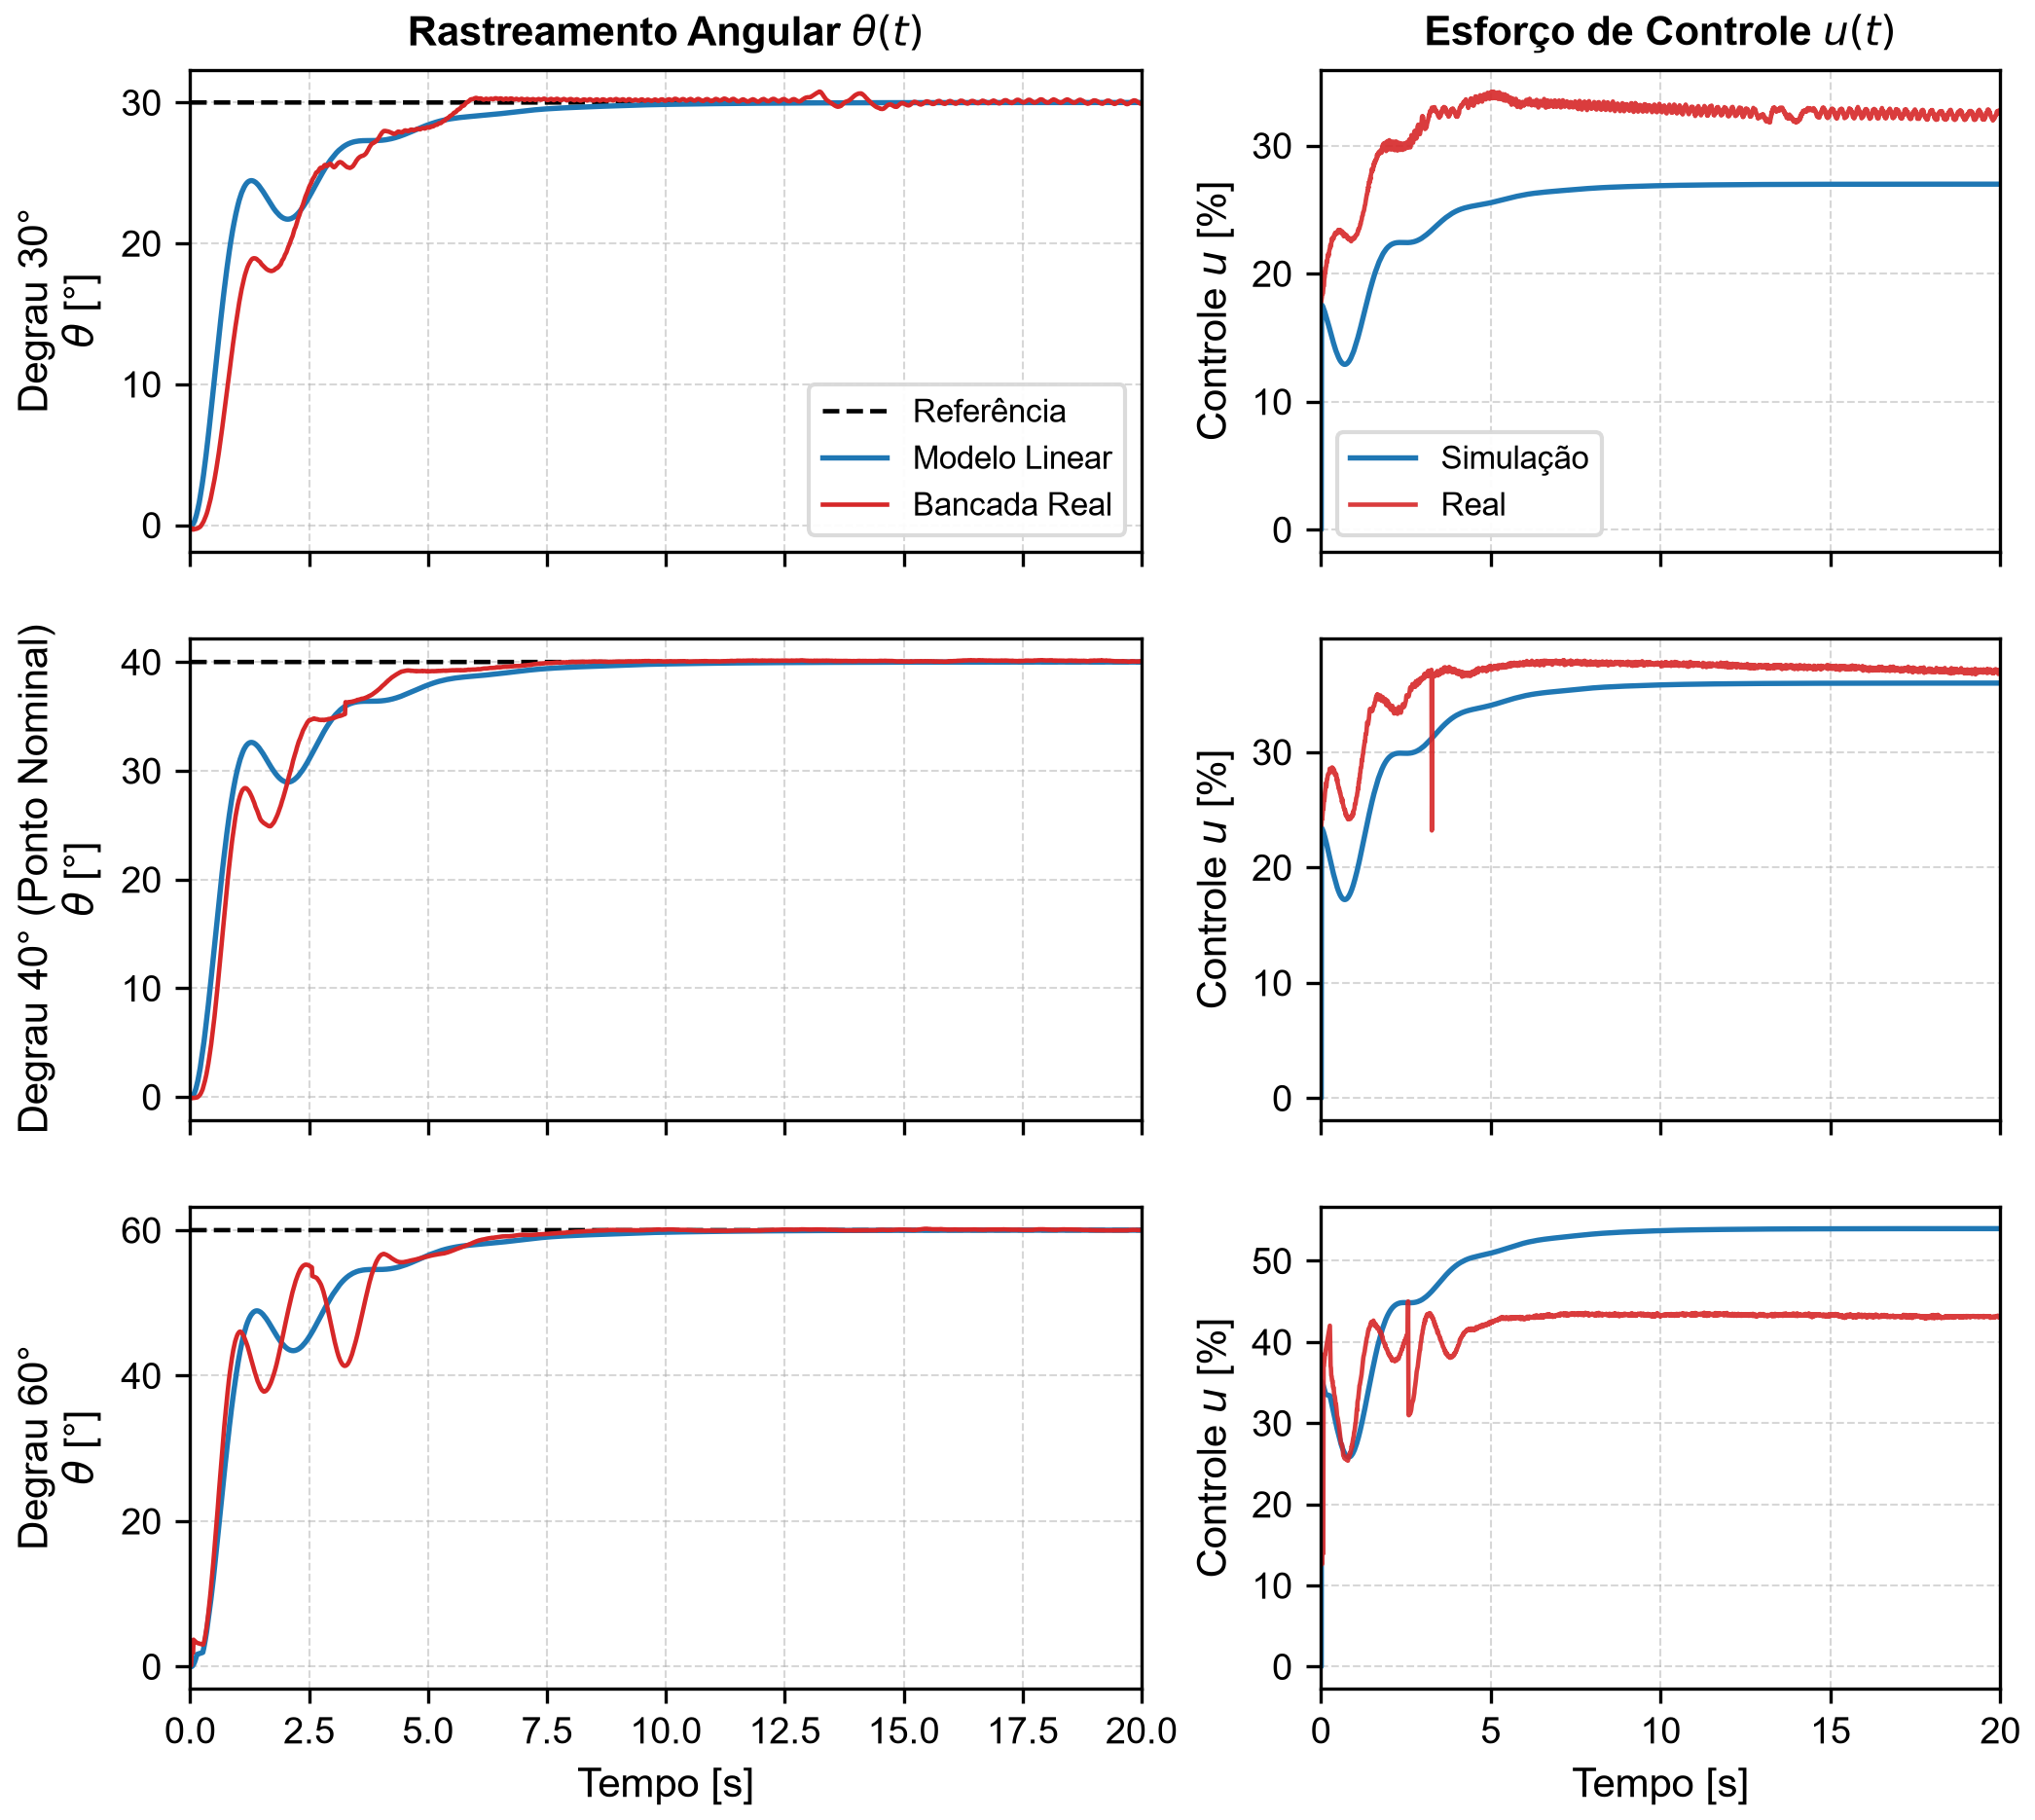
\includegraphics[width=0.95\textwidth]{img/pid_degraus_consolidado.png}
    \sourceFig{o autor, 2026.}
\end{figure}

A análise comparativa da Figura~\ref{fig:pid_degraus_consolidado} revela aspectos fundamentais da dinâmica do aeropêndulo:
\begin{itemize}
    \item \textbf{Ponto Nominal ($40^\circ$):} No patamar em torno do qual o modelo linear foi sintonizado, observa-se alta concordância entre a resposta simulada e a real. O erro transitório de modelagem permanece inferior a $\pm 6^\circ$ durante a subida, atingindo regime permanente em torno de 5\,s com erro estacionário nulo e esforço de controle praticamente idêntico ($u_{\text{sim}} = 35{,}98\%$ contra $u_{\text{real}} = 36{,}83\%$);
    
    \item \textbf{Assimetria e Variação de Ganho Estático ($30^\circ$ e $60^\circ$):} À medida que a referência se afasta do ponto nominal, manifesta-se a severa não-linearidade da planta. Em $30^\circ$, o empuxo contínuo exigido para equilíbrio é de $32{,}61\%$, enquanto o modelo linear prediz $26{,}98\%$ (discrepância de $5{,}63\%$ de duty cycle). Em $60^\circ$, onde a componente gravitacional restauradora $(m_1 L_1 - m_2 L_2)g\sin(\theta)$ impõe máxima resistência, o esforço real exigido atinge $42{,}74\%$, divergindo dos $53{,}97\%$ calculados linearmente (erro de ganho estático superior a $11\%$ de duty cycle);
    
    \item \textbf{Diferenças de Dinâmica Transitória:} A resposta real em $60^\circ$ apresenta amortecimento superior ao previsto pelo modelo linear em virtude do aumento do arrasto aerodinâmico induzido pela hélice em altas rotações.
\end{itemize}

Essa disparidade comprova experimentalmente que um modelo linear invariante no tempo e um controlador linear clássico (PID) são incapazes de garantir desempenho homogêneo ao longo de todo o envelope de voo do aeropêndulo. Esse resultado justifica plenamente a necessidade de adotar uma formulação preditiva não-linear (NMPC) baseada em modelo dinâmico NARX, apresentada a seguir.
% ------------------------------------------------------------
\subsection{Formulação do NMPC}
\label{subsec:nmpc_ocp}

O NMPC fundamenta-se na resolução repetida, a cada período de amostragem $T_s$, de um Problema de Controle Ótimo (OCP) em horizonte finito \cite{rawlings2017}. A síntese offline desse controlador exige ferramentas capazes de (i)~expressar simbolicamente o modelo dinâmico não-linear, (ii)~transcrever o OCP em um Problema de Programação Não-Linear (NLP) e (iii)~calcular automaticamente as derivadas de primeira e segunda ordem exigidas pelo resolvedor numérico. O framework CasADi atende a esses três requisitos de forma integrada \cite{andersson2019}.

\subsubsection*{Problema de Controle Ótimo em Horizonte Finito}

Para o estado atual $x_k$ e a referência $x_{ref,k} = [\theta_{ref,k},\; 0]^\top$, define-se o conjunto de sequências de controle admissíveis
\begin{equation}
    \mathcal{U}_N(x_k) := \bigl\{U_k \mid
        (x_{k+j|k},\, u_{k+j}) \in \mathcal{Z},\;
        x_{k+N|k} \in \mathcal{X}_f,\;
        j = 0,\ldots,N-1
    \bigr\},
    \label{eq:admissivel}
\end{equation}
\noindent onde $\mathcal{Z} := \mathcal{X} \times \mathcal{U}$ é o conjunto admissível de pares estado-controle e $\mathcal{X}_f \subseteq \mathcal{X}$ é o conjunto terminal. O domínio de factibilidade do OCP é
\begin{equation}
    \mathcal{X}_N := \bigl\{x \in \mathcal{X} \mid
        \mathcal{U}_N(x) \neq \emptyset \bigr\},
    \label{eq:factivel}
\end{equation}
\noindent ou seja, o conjunto de estados a partir dos quais existe ao menos uma sequência de controle que satisfaz todas as restrições e conduz o sistema ao conjunto terminal em $N$ passos \cite{rawlings2017}.

O OCP resolvido no instante $k$ é
\begin{equation}
    \min_{U_k}\;
    \underbrace{\sum_{j=0}^{N-1}
    \ell\!\left(x_{k+j|k},\, u_{k+j},\, x_{ref,k}\right)}_{\text{custo acumulado}}
    +\;
    \underbrace{V_f\!\left(x_{k+N|k},\, x_{ref,k}\right)}_{\text{custo terminal}}
    \label{eq:ocp}
\end{equation}
\noindent sujeito a
\begin{align}
    x_{k+j+1|k} &= x_{k+j|k} + T_s\, f\!\left(x_{k+j|k},\, u_{k+j}\right),
    && j = 0, \ldots, N-1, \label{eq:ocp_dinamica} \\
    x_{k|k}      &= x_k, \label{eq:ocp_ic} \\
    u_{k+j}      &\in \mathcal{U}, && j = 0, \ldots, N-1, \label{eq:ocp_u} \\
    x_{k+j|k}    &\in \mathcal{X}, && j = 1, \ldots, N, \label{eq:ocp_x} \\
    x_{k+N|k}    &\in \mathcal{X}_f, \label{eq:ocp_terminal}
\end{align}
\noindent onde $N$ é o horizonte de predição; $U_k = \{u_{k}, \ldots, u_{k+N-1}\}$ é a sequência de controle a otimizar; $x_{k+j|k}$ é o estado predito $j$ passos à frente, propagado pela discretização de Euler explícita da dinâmica contínua~\eqref{eq:estadonl}; e $\mathcal{U}$ e $\mathcal{X}$ são os conjuntos admissíveis de entrada e de estado.

\subsubsection*{Custo de Estágio e Custo Terminal}

O custo de estágio adota a forma quadrática em relação ao vetor de estados completo $x = [\theta,\; \dot{\theta}]^\top$ e ao vetor de referência $x_{ref} = [\theta_{ref},\; 0]^\top$:
\begin{equation}
    \ell(x, u, x_{ref}) =
    (x - x_{ref})^\top Q\,(x - x_{ref}) + u^\top R\, u,
    \label{eq:custo_estagio}
\end{equation}
\noindent onde $Q \in \mathbb{R}^{2\times2}$ e $R \in \mathbb{R}$ são, respectivamente, as matrizes de peso definidas positivas ($Q \succ 0$ e $R > 0$). A matriz $Q$ penaliza o erro de rastreamento angular e a velocidade angular, garantindo o amortecimento do sistema, enquanto $R$ penaliza o esforço de controle, inibindo variações bruscas no sinal enviado ao ESC. A positividade estrita de $Q$ e $R$ garante que $\ell(x, u, x_{ref}) \geq \alpha_1(|x - x_{ref}|)$ para alguma função de classe $\mathcal{K}_\infty$, condição necessária para que a função de valor ótimo $V_N^0(\cdot)$ admita uma cota inferior compatível com os requisitos de uma função de Lyapunov \cite{rawlings2017}.


O custo terminal é definido de forma análoga sobre o vetor de estados:
\begin{equation}
    V_f(x, x_{ref}) =
    (x - x_{ref})^\top P\,(x - x_{ref}),
    \label{eq:custo_terminal}
\end{equation}
\noindent onde a matriz $P \succ 0$ é obtida pela solução da equação de Lyapunov do sistema linearizado em torno do ponto de equilíbrio, operando sob uma lei de controle local estabilizante $u = K(x - x_{ref})$. Essa escolha garante que $V_f$ atue como uma Função de Lyapunov de Controle (CLF) local: para todo $x \in \mathcal{X}_f$, existe $u = Kx$ tal que
\begin{equation}
    V_f\!\left(f(x, u),\, x_{ref}\right) - V_f(x, x_{ref})
    \leq -\ell(x, u, x_{ref}),
    \label{eq:clf}
\end{equation}
\noindent condição denominada suposição básica de estabilidade por
\citeonline{rawlings2017}. O conjunto terminal
$\mathcal{X}_f$ é escolhido como um subconjunto compacto e invariante por
controle em torno de $\theta_{ref}$, tipicamente um subnível de $V_f$, de
modo que~\eqref{eq:clf} seja satisfeita para todo $x \in \mathcal{X}_f$.

\subsubsection*{Estratégia de Horizonte Deslizante e Viabilidade Recursiva}

A estratégia de horizonte deslizante (\textit{receding horizon}) aplica apenas a primeira ação ótima $u_k^* = u^0(0; x_k)$ da sequência $U_k^* = \arg\min \eqref{eq:ocp}$, descarta os demais elementos e resolve novamente o OCP no instante seguinte com o novo estado medido $x_{k+1}$, incorporando retroalimentação de forma natural \cite{mayne2000}. A lei de controle implícita resultante é
\begin{equation}
    \kappa_N(x_k) := u^0(0;\, x_k), \qquad x_k \in \mathcal{X}_N.
    \label{eq:lei_controle}
\end{equation}

Uma propriedade fundamental dessa estratégia é a viabilidade recursiva, se o OCP é factível para o estado inicial $x_0 \in \mathcal{X}_N$, então ele permanece factível para todos os estados subsequentes $x_k$ do sistema em malha fechada $x^+ = f(x,
\kappa_N(x))$, desde que $\mathcal{X}_f$ seja invariante por controle \cite{rawlings2017}. Isso garante que o controlador nunca encontra um estado para o qual não exista solução, evitando falhas em operação.
Sob as condições~\eqref{eq:clf}, pode-se mostrar que a função de valor ótimo satisfaz
\begin{equation}
    V_N^0\!\left(f(x, \kappa_N(x))\right) \leq V_N^0(x) - \ell(x,\kappa_N(x))
    \quad \forall x \in \mathcal{X}_N,
    \label{eq:descida}
\end{equation}
\noindent o que caracteriza $V_N^0(\cdot)$ como uma função de Lyapunov do sistema em malha fechada, assegurando estabilidade assintótica da origem (erro de rastreamento nulo) em $\mathcal{X}_N$ \cite{rawlings2017}.

O OCP~\eqref{eq:ocp}--\eqref{eq:ocp_terminal} é transcrito em um NLP e resolvido pelo CasADi \cite{andersson2019}, que constrói grafos de expressão simbólica (DAGs) e calcula automaticamente as derivadas de primeira e segunda ordem exigidas pelo resolvedor numérico IPOPT.

% ------------------------------------------------------------
\subsection{Geração do \textit{Dataset}}

A política de controle ótima gerada pelo NMPC em malha fechada é utilizada para compor o \textit{dataset} de treinamento da rede neural MLP, conforme o bloco central da fase offline na Figura~\ref{fig:diagrama-blocos-projeto}. Para cada instante de simulação, o OCP~\eqref{eq:ocp} é parametrizado pela referência corrente $\theta_{ref,k}$, e registra-se o par entrada-saída:
\begin{equation}
    \mathcal{D} = \bigl\{
        \bigl(x_k,\; u_k^*\bigr)
    \bigr\}_{k=1}^{M},
    \label{eq:dataset}
\end{equation}
\noindent onde $x_k \in \mathbb{R}^{130}$ denota o vetor de características composto pelas $n_y = 15$ saídas passadas da planta ($\theta_{k-1}, \dots, \theta_{k-15}$), pelas $n_u = 15$ ações de controle passadas ($u_{k-1}, \dots, u_{k-15}$) e pelos $N = 100$ passos de referência futura no horizonte de predição ($\theta_{\text{ref}, k}, \dots, \theta_{\text{ref}, k+N-1}$), e $u_k^* \in \mathbb{R}$ representa a ação de controle ótima obtida da solução do OCP em malha fechada.

A inclusão das referências futuras dota a rede neural da capacidade de visão antecipada (\textit{preview}), permitindo compensar preventivamente a inércia mecânica da planta, em harmonia com a formulação do OCP da Seção~\ref{subsec:nmpc_ocp}. Para alimentar a resolução offline do controlador ótimo e assegurar rica cobertura do espaço de estados, sintetizou-se uma trajetória multivariada com duração de 187\,s, combinando trechos senoidais harmônicos até $0{,}50$\,Hz com degraus de amplitude comutada que percorrem desde $12^\circ$ até $110^\circ$, cobrindo dinâmicas de transição e regimes estáticos ao longo de todo o envelope operacional \cite{karg2020}.

O \textit{dataset} é normalizado componente a componente para o intervalo $[-1, 1]$ antes do treinamento, procedimento padrão que melhora o condicionamento do problema de otimização do aprendizado e a convergência do algoritmo Adam \cite{karg2020}.

% ------------------------------------------------------------
\subsection{Arquitetura e Treinamento da MLP}

A implementação e o treinamento da rede neural MLP são realizados utilizando o PyTorch. O PyTorch é uma biblioteca de aprendizado de máquina que unifica facilidade de uso e alta performance computacional. Diferentemente de frameworks baseados na construção prévia de grafos estáticos de fluxo de dados, o PyTorch adota o paradigma de execução dinâmica e imperativa. Isso permite que os modelos de aprendizado profundo sejam programados e depurados como programas Python convencionais, mantendo o controle total do fluxo sob responsabilidade do usuário \cite{paszke2019}.
A estrutura da rede, a configuração dos hiperparâmetros e a rotina de otimização, que inclui um critério de parada prematura (\textit{early stopping}) para evitar \textit{overfitting}, estão consolidadas no Algoritmo~\ref{alg:treino_mlp}.

\begin{algorithm}
\caption{Treinamento da Rede Neural para Aproximação do Controlador}
\label{alg:treino_mlp}
\begin{algorithmic}[1]

\Procedure{TreinarAproximador}{}

    \State Carregar dataset gerado pelo controlador ótimo
    \State Dividir dataset em conjuntos de treino, validação e teste
    \State Inicializar rede neural e otimizador
    \State $melhorLoss \gets \infty$, \quad $contadorPaciencia \gets 0$

    \Statex
    \For{cada época}
        \State Atualizar pesos minimizando o erro nos batches de treino
        \State Avaliar erro no conjunto de validação

        \If{houve melhora na validação}
            \State Registrar melhora e salvar pesos atuais
            \State Resetar contador de paciência
        \Else
            \State Incrementar contador de paciência
            \If{paciência esgotada}
                \State \textbf{break} \Comment{\textit{Early stopping}}
            \EndIf
        \EndIf
    \EndFor

    \Statex
    \State Restaurar melhores pesos
    \State Avaliar desempenho final no conjunto de teste
    \State Exportar modelo para implantação embarcada

\EndProcedure
\end{algorithmic}
\end{algorithm}

% ============================================================
\section{Controle Embarcado em Tempo Real}
\label{sec:embarcado}

% ------------------------------------------------------------
\subsection{Conversão via X-CUBE-AI}

O STM32Cube.AI é uma ferramenta de software desenvolvida pela STMicroelectronics projetada para a implantação de aprendizado de máquina em microcontroladores (TinyML). Esse ecossistema atua como um gerador de código baseado em compilação, recebendo modelos treinados em plataformas como Keras e TensorFlow Lite para gerar código C otimizado para a linha de microcontroladores STM32 \cite{stmu2526}.

Diferentemente de abordagens baseadas em interpretadores embarcados, que processam a topologia do modelo em tempo de execução, a geração de código nativo pode aumentar consideravelmente o desempenho da inferência. Como apontado por \citeonline{david2021}, metodologias baseadas em compilação fixam as chamadas de operação diretamente em código de máquina, eliminando as etapas de roteamento do interpretador. A ferramenta analisa a topologia da rede neural, otimiza o uso de \textit{buffers} e mapeia as operações matemáticas diretamente para as capacidades de hardware do processador alvo, minimizando o uso de memória Flash e SRAM e permitindo a execução de inferências com restrições de latência e consumo energético.

% ------------------------------------------------------------
\subsection{Firmware de Controle no STM32}

O firmware de controle utiliza uma arquitetura orientada a eventos e não-bloqueante para garantir o atendimento ao \textit{deadline} de $T_s = 10$\,ms. Um temporizador de hardware (TIM) operando a 100\,Hz atua como base de tempo determinística. A cada disparo do timer, a CPU apenas inicia a transferência dos dados inerciais da IMU via I$^2$C utilizando acesso direto à memória (DMA) e retorna imediatamente do contexto de interrupção, não bloqueando a execução.

Apenas quando a transferência I$^2$C é concluída, uma interrupção de conclusão do DMA (\textit{Transfer Complete}) é acionada, desencadeando a rotina de controle principal. Neste momento, com os dados inerciais já disponíveis na memória SRAM, o processador realiza a leitura da referência angular, a estimação do estado atual via filtro complementar, a inferência da rede neural e a atualização do \textit{duty cycle} do PWM no ESC, conforme o Algoritmo~\ref{alg:isr_controle}.

As operações de ponto flutuante, em particular o cálculo de \texttt{atan2} no filtro complementar e as multiplicações matriciais da MLP gerada pelo X-CUBE-AI, são executadas nativamente pela FPU do Cortex-M4, eliminando a sobrecarga de emulação por software. A transmissão da telemetria ao final da rotina também é delegada a um canal DMA vinculado à UART. Essa delegação maciça da movimentação de dados aos periféricos garante que o tempo de CPU fique dedicado estritamente aos cálculos de controle.

\begin{algorithm}[H]
\caption{Rotina de Controle em Tempo Real (Arquitetura DMA)}
\label{alg:isr_controle}
\begin{algorithmic}[1]
\Statex \textbf{Base de Tempo:} $f_s = 100$\,Hz ($T_s = 10$\,ms)
\Statex

\Procedure{Timer\_ISR}{}
    \State \Comment{Disparo determinístico a cada 10ms}
    \State $\text{IniciarLeituraIMU\_DMA()}$ \Comment{Inicia transação I$^2$C em background}
\EndProcedure

\Statex
\Procedure{I2C\_DMA\_Complete\_ISR}{}
    \State \Comment{1. Leitura da Referência (UART)}
    \State $\theta_{ref} \gets \text{LerReferencia()}$

    \Statex
    \State \Comment{2. Estimação de Estados (FPU)}
    \State $\theta, \dot{\theta} \gets \text{EstimarEstados(Buffer\_I2C)}$

    \Statex
    \State \Comment{3. Cálculo da Ação de Controle (Inferência Neural)}
    \State $x_{\text{in}} \gets \text{MontarVetorEntrada}(\theta_{\text{hist}},\, u_{\text{hist}},\, r_{\text{futuro}})$ \Comment{130 variáveis com \textit{preview}}
    \State $u \gets \text{InferirMLP}(x_{\text{in}})$

    \Statex
    \State \Comment{4. Atuação (PWM)}
    \State $\text{AplicarControle}(u)$

    \Statex
    \State \Comment{5. Registro de Dados (UART DMA)}
    \State $\text{IniciarTelemetria\_DMA}(\theta,\; \dot{\theta},\; \theta_{ref},\; u)$
\EndProcedure
\end{algorithmic}
\end{algorithm}
% ============================================================
